```latex
\documentclass[12pt,a4paper]{article}
\usepackage[utf8]{inputenc}
\usepackage{xcolor}
\usepackage{tikz}
\usepackage[margin=1in]{geometry}

\newcommand{\bitstuff}[1]{\textcolor{red}{\textbf{#1}}}

\begin{document}

\begin{center}
\textbf{Computer Networks Examination (5 marks)}
\\\vspace{0.25cm}
\textit{Bit Stuffing Problem}
\end{center}

\textbf{Question:} What would be the bit pattern of the following bit stream after "Bit Stuffing"? Please indicate the stuffed bit. \texttt{0101011111101000000101111101}

\textbf{Answer:}

1. \textbf{Bit Stuffing Explanation (2-3 lines):}
   Bit stuffing is a technique used in data link layer protocols to prevent pattern sensitivity. It involves inserting a '0' bit after every sequence of five consecutive '1' bits in the data stream. This ensures that control sequences (like flags) are not accidentally replicated within the data.

2. \textbf{Solution:}
   Original stream: \texttt{0101011111101000000101111101}
   
   After bit stuffing:
   \begin{center}
   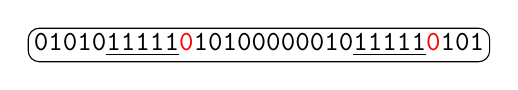
\begin{tikzpicture}
   \node[draw,rounded corners,inner sep=2pt] {
   \texttt{01010\underline{11111}\bitstuff{0}10100000010\underline{11111}\bitstuff{0}101}
   };
   \end{tikzpicture}
   \end{center}

3. \textbf{Explanation:}
   - First \texttt{11111} sequence: \texttt{01010\underline{11111}} → Insert \bitstuff{0}
   - Second \texttt{11111} sequence: \texttt{...010\underline{11111}} → Insert \bitstuff{0}
   - No more sequences of five consecutive '1' bits remain

4. \textbf{Final Result:}
   \texttt{0101011111\bitstuff{0}101000000101111\bitstuff{0}101}

   \textit{Note: \textcolor{red}{\textbf{Red}} bits are the stuffed bits.}

\end{document}
```